\documentclass[12pt]{article}
\usepackage{amsmath}
\usepackage{graphicx}
\usepackage{hyperref}
\usepackage[latin1]{inputenc}

\title{Hidden Markov Model}
\author{Da Huo}
\date{08/15/2018}

\begin{document}
\maketitle

This is the Hidden Markov Model we constructed for predicting the probability of The Coffee Pot is empty. In this model, the state $X$ is whether the pot is empty. $X=\{E,\neg E\}$ The observation $r$ here is how many times the pot is been removed. $R=\{1,2,...,n\}$ where n is the last time coffee pot been removed in one coffee making cycle. When we detect the coffee machine is on again, we reset $r$ and count from 1 again.

\begin{figure}[!htbp]
\center
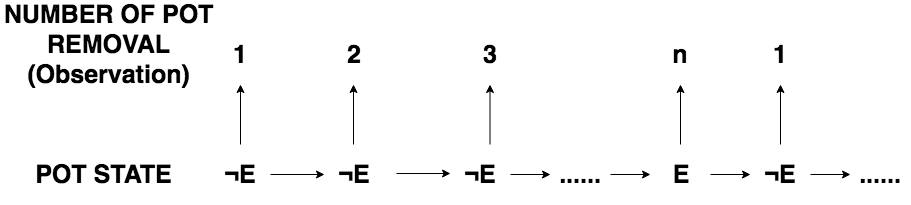
\includegraphics[scale=0.4]{figure0}
\caption{HMM of Coffee Predicting}
\end{figure}

\section*{Priors in Inference}

\subsection*{Transition Model}

\begin{equation}
P(X_{t+1}=E|X_{t}=E)=0
\end{equation}
Here, we assume the when pot is empty, the next time we receive a data point is when making coffee is detected and coffee pot is definitely not empty.

\begin{equation}
P(X_{t+1}=E|X_{t}=\neg E)=\frac{1}{\text{\# of pot removals within one cycle of making coffee}}
\end{equation}

\subsection*{Sensor Model}
\begin{equation}
P(R_{t}=n|X_{t}=E)=\frac{\text{\# of } R \geq n|E}{\text{\# of E}}
\end{equation}

\begin{equation}
P(R_{t}=n|X_{t}=\neg E)=\frac{\text{\# of } R \geq n|\neg E}{\text{\# of } \neg E}
\end{equation}

\section*{Inference}
\subsection*{Transition Matrix}
\begin{equation}
T=
\begin{bmatrix}
    P(X_{t+1}=E|X_{t}=E) & P(X_{t+1}=\neg E|X_{t}=E) \\
    P(X_{t+1}=E|X_{t}=\neg E) &P(X_{t+1}=\neg E|X_{t}=\neg E) \\

\end{bmatrix}
\end{equation}
\subsection*{Observation Matrix}
\begin{equation}
O_{R=n}=
\begin{bmatrix}
    P(R_{t}=n|X_{t}=E) & 0 \\
    0 &P(R_{t}=n|X_{t}=\neg E) \\

\end{bmatrix}
\end{equation}

\subsection*{Inference}
Let $f_{i}=P(X_{i})$,
\begin{equation}
f_{t+1}=\alpha f_{t}TO_{R_{t+1}=n}
\end{equation}








\end{document}
